% LTeX: language=en-GB
% \documentclass[aspectratio=169]{beamer}
\documentclass[aspectratio=169, handout]{beamer}
\usetheme{Arguelles}
\usepackage[utf8]{inputenc}
\usepackage[T1]{fontenc}
\usepackage[english]{babel}
\usepackage{nth}
\usepackage{graphicx}
\usepackage{pgfgantt}
\usepackage{tikz}
\usepackage{booktabs}

% -------------------------- Define Beamer options ----------------------------

\definecolor{DTUred}{cmyk}{0, .91, .72, .23}
\definecolor{itemcolor}{cmyk}{0,0,0,0.56}
\definecolor{blockbodycolor}{cmyk}{0,1,1,0.5}
\definecolor{White}{cmyk}{0,0,0,0}
\setbeamercolor*{structure}{fg=DTUred}
\setbeamercolor*{frametitle}{fg=DTUred}
\setbeamercolor*{redbox}{fg=White, bg=blockbodycolor}

% ---------------------------------- Beamer: ----------------------------------

\title{Verification of digital circuits using Java}
\subtitle{Bachelor's project}
\author{Rasmus Wiuff}
\institute{DTU}
\date{\nth{19} of May 2025}

\begin{document}

\frame[plain]{\titlepage}

\begin{frame}{Outline}
    \tableofcontents
\end{frame}

\section{Introduction}
\begin{frame}{Introduction}
    \begin{itemize}
        \item Chip design requires verification
        \item Verification most commonly done using UVM
        \item Commonly used frameworks: Chisel, SpinalHDL, pyuvm
        \item ABV and formal verification improves the verification step
    \end{itemize}
    \begin{center}
        \begin{tabular}{l}
            \toprule
            Verification cycles reduced by 25-30\%             \\
            Pre-silicon bug detection rates improved by 20\%   \\
            Security vulnerability detection increased by 40\% \\
            \bottomrule
        \end{tabular}
    \end{center}
\end{frame}
\section{Problem specification}
\begin{frame}{Problem specification}
    \begin{center}
        \begin{beamercolorbox}[sep=2em]{redbox}
            \textbf{A chip verification framework written in Java, supporting SystemVerilog and core ideas from ABV, thus making it easy for designers to write their designs in SystemVerilog and use a well known language to implement assertion based tests.}
        \end{beamercolorbox}
        \begin{tabular}{ll}
            \toprule
            Challenge         & Success Criteria                             \\
            \midrule
            Simulation driver & Launching and handling output from Verilator \\
            Peek-poke-step    & Basic verification tests                     \\
            Assertions        & SVA assertions                               \\
            Test-translation  & Translate tests into a testbench             \\
            Concurrency       & Concurrent execution of the tests            \\
            \bottomrule
        \end{tabular}
    \end{center}
\end{frame}
\section{Design}
\begin{frame}{Usecases}
    \begin{columns}
        \begin{column}{.45\textwidth}
            \begin{itemize}
                \item Adding devices
                \item Adding tests
                \item Configuring tests
                \item Run simulations
            \end{itemize}
        \end{column}
        \begin{column}{.45\textwidth}
            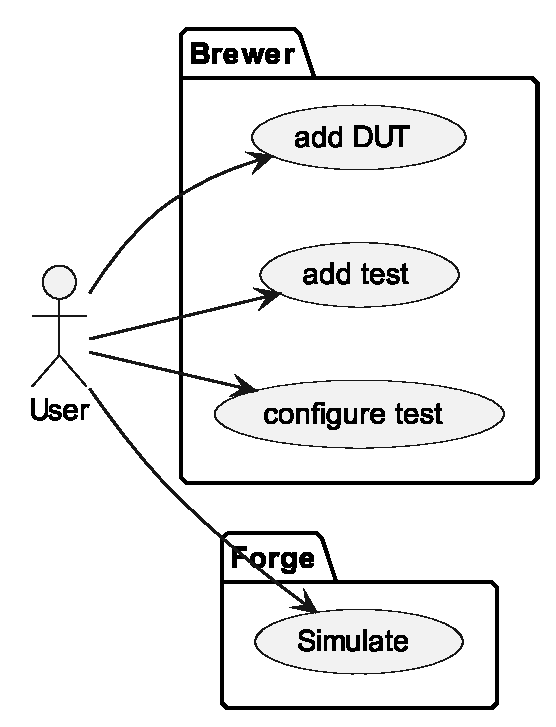
\includegraphics[width=.8\columnwidth]{out/plantuml/usecase2/usecase2.eps}
        \end{column}
    \end{columns}
\end{frame}
\begin{frame}{Separation of responsibility}
    \begin{columns}[T]
        \begin{column}{.45\textwidth}
            \textbf{The Brewer}
            \begin{itemize}
                \item Adding devices
                \item Handling test logic
                \item Preparing testbenches
            \end{itemize}
        \end{column}
        \begin{column}{.45\textwidth}
            \textbf{The Forge}
            \begin{itemize}
                \item Define command arguments
                \item Launch Verilator
                \item Collect Verilator output
                \item Handle concurrency
            \end{itemize}
        \end{column}
    \end{columns}
\end{frame}
\begin{frame}{The final workflow}
    \begin{center}
        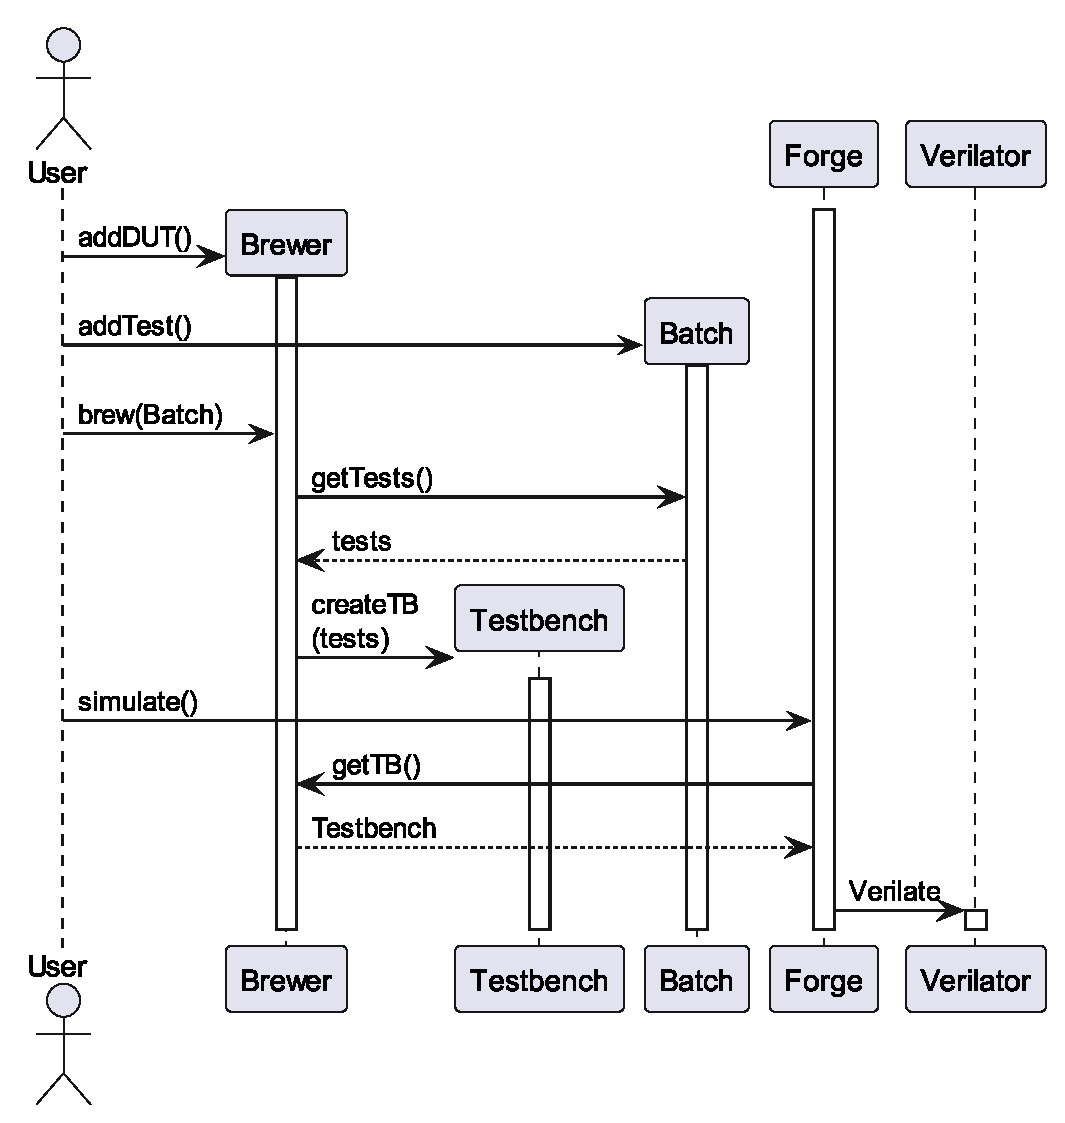
\includegraphics[height=.8\textheight]{out/plantuml/seq/sequenceDiag.eps}
    \end{center}
\end{frame}
\section{Implementation}
\begin{frame}{The program structure}
    \begin{center}
        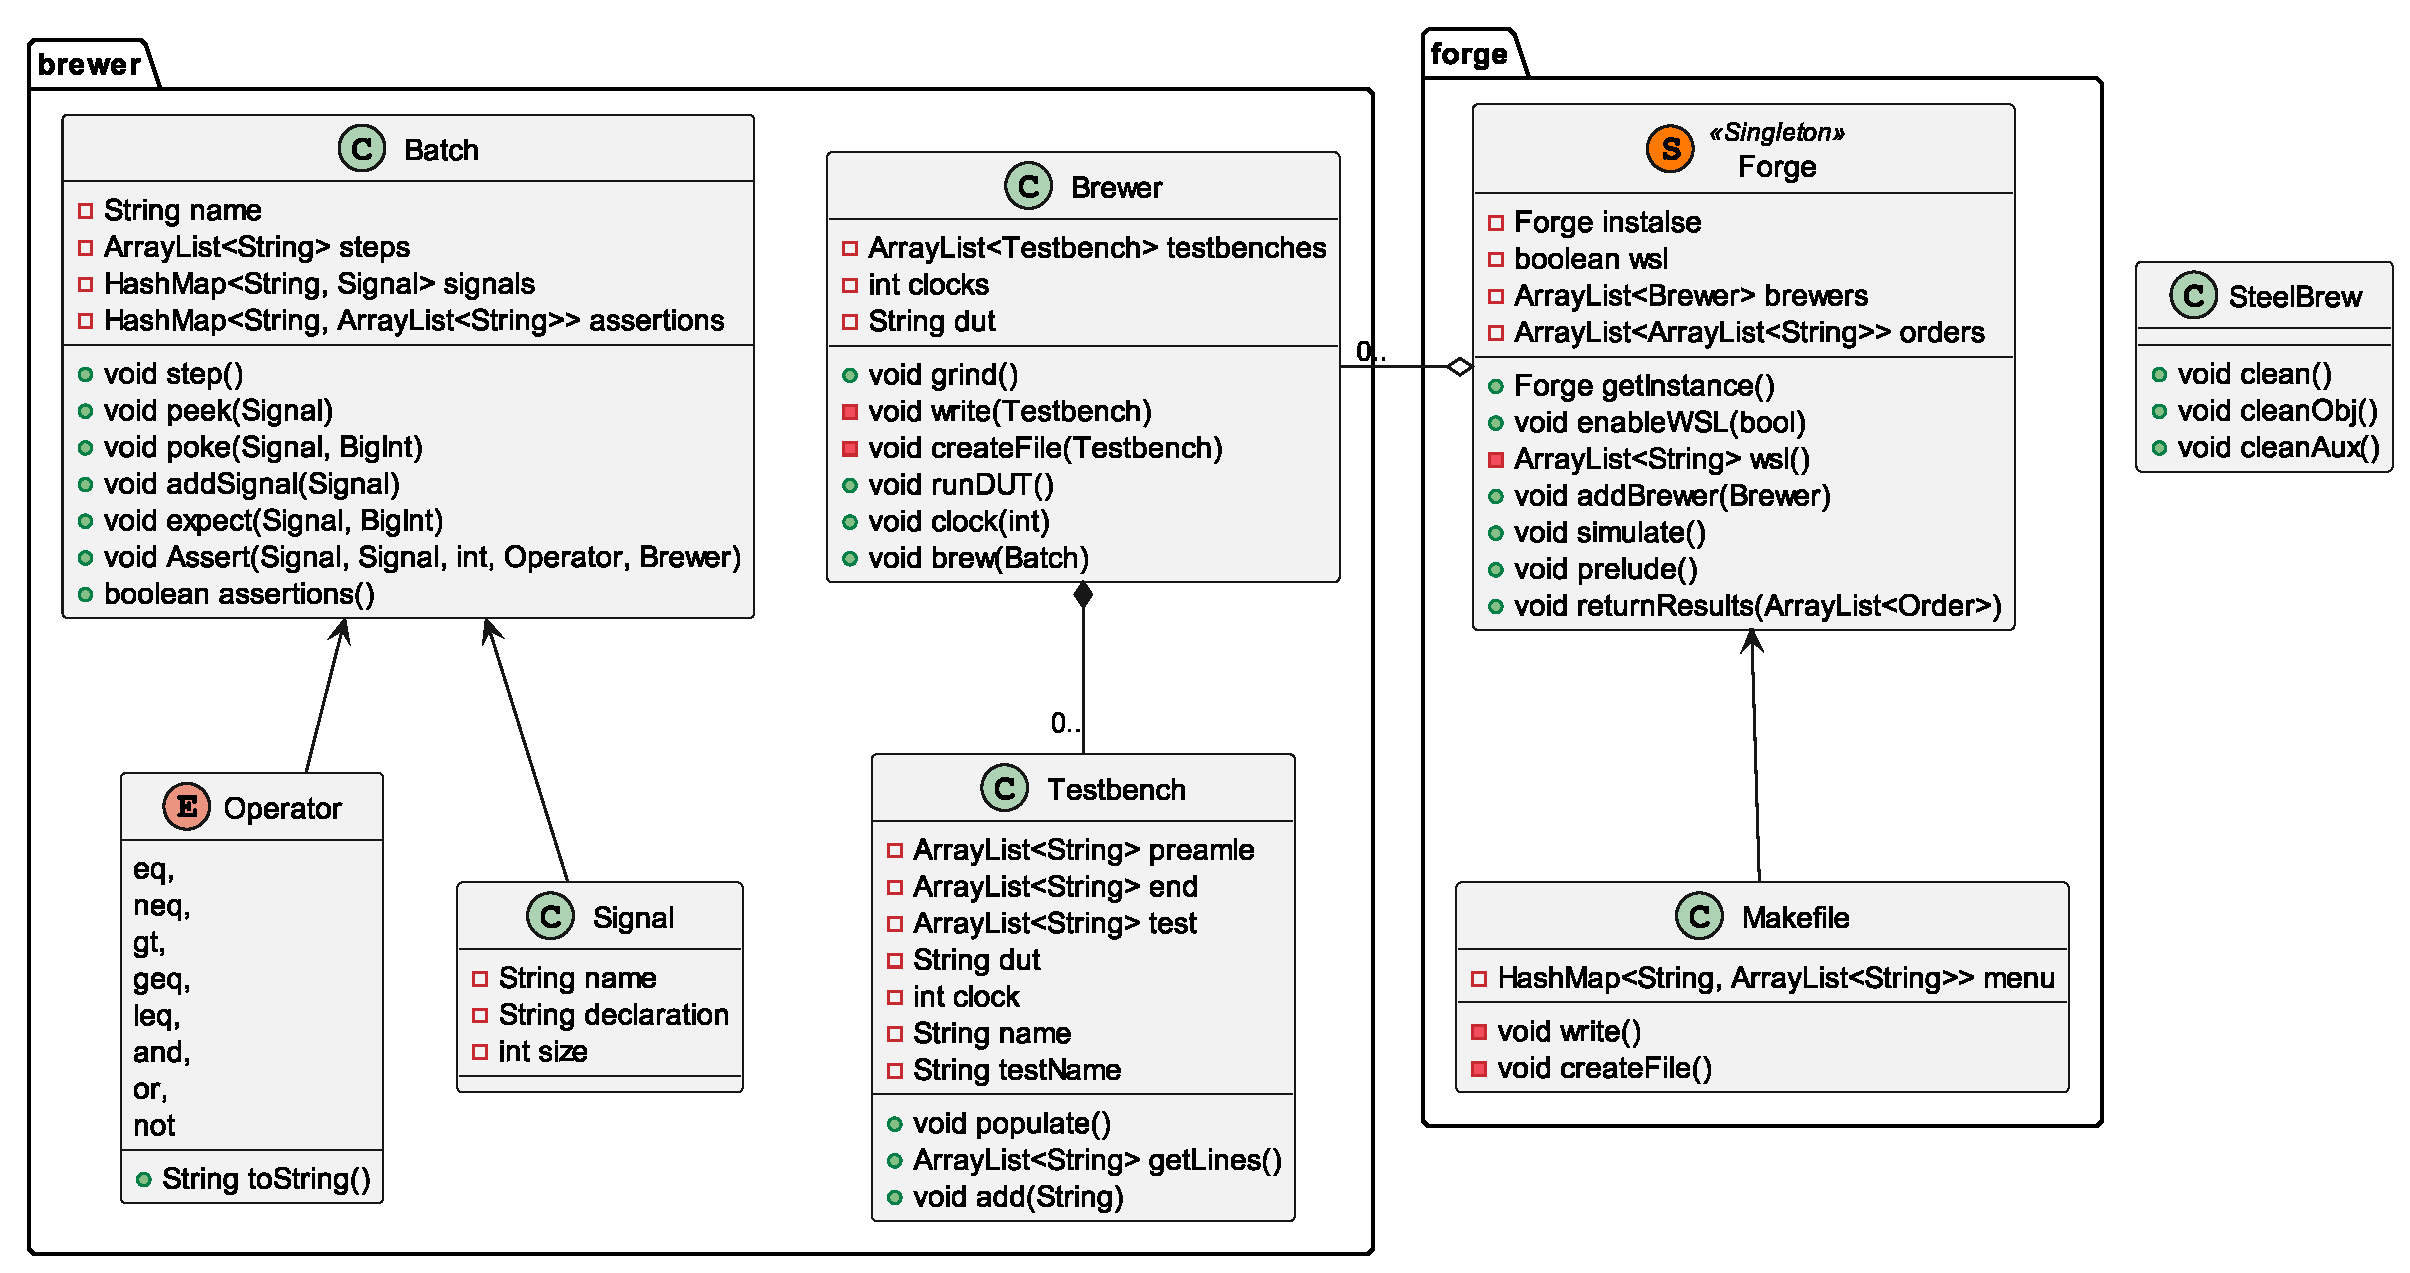
\includegraphics[height=.8\textheight]{out/plantuml/classDiag/classDiag.eps}
    \end{center}
\end{frame}
\begin{frame}{Defining tests}
    
\end{frame}
\begin{frame}{Running tests}
    
\end{frame}
\section{Result}
\begin{frame}{Using the project}

\end{frame}
\section{Further development}
\begin{frame}{Further development}

\end{frame}
\section{Conclusion}
\begin{frame}{Conclusion}

\end{frame}
\section*{}
\begin{frame}[plain,standout]{Q\&A}
    \begin{columns}
        \begin{column}{.3\textwidth}
            \begin{center}
                Questions?
            \end{center}
        \end{column}
        \begin{column}{.5\textwidth}
            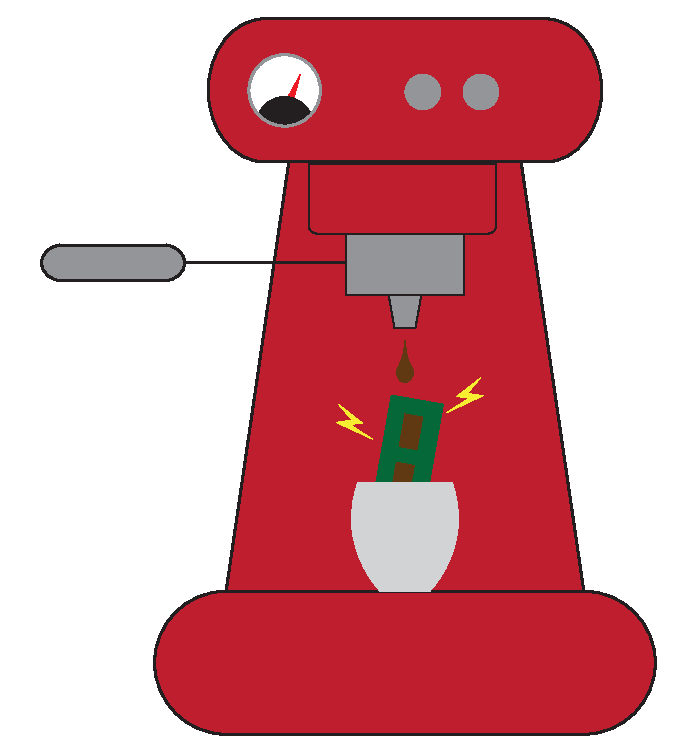
\includegraphics[width=.8\columnwidth]{graphics/steelbrew.eps}
        \end{column}
    \end{columns}
\end{frame}
\end{document}